\section{Travail déjà réalisé dans BlueBanana}
	\label{BlueBanana}
	La mobilité des avatars implique de nombreux échanges de données à travers le réseau pair à pair. Comme les overlays de l'état de l'art n'anticipent pas cette mobilité, les données nécessaires ne seront pas chargées à temps, ce qui conduit à des défaillances transitoires au niveau applicatif. Blue Banana a été réalisé pour résoudre ce problème, il modélise et prédit les mouvements des avatars ce qui permet à l'overlay de s'adapter par anticipation aux besoins du jeux.
	\subsection{Explications}
	Blue Banana est implémenté au dessus de Sollipsis que l'on a pu étudier auparavant. Une des premières innovations qui a été introduite est la distinction de plusieurs états d'un avatar. Car comme il a été possible de voir dans la partie sur la collecte de trace, un avatar se comporte différemment en fonction des zones du monde. Deux états ont donc été introduit:
	\begin{itemize}
		\item \textbf{T}(ravelling): l'avatar se déplace rapidement sur la carte et il a une trajectoire droite.  
		\item \textbf{E}(xploring): l'avatar est en train d'explorer une zone, sa trajectoire est confuse et sa vitesse est lente.
	\end{itemize} 
	Le changement d'état se fait en fonction de la vitesse de l'avatar, si la vitesse devient supérieur à une borne et que l'avatar est dans l'état E alors l'avatar passe en état T. Ce modèle pourra être affiné par la suite en prenant en compte l'accélération ou l'historique des mouvements. \\
	Un autre mécanisme a été mis en place, il s'agit d'anticiper les mouvements d'un avatar, pour cela deux suppositions sont faites: seulement une prédiction courte est cohérente et plus l'avatar se déplace rapidement, plus il y a de chance qu'il continue dans la même direction. Comme nous pouvons voir sur le schéma ~\ref{Propa_Algo}, en fonction du vecteur de mouvement de l'avatar, le système va rapatrier les données des nœuds qui se trouvent sur la trajectoire probable de l'avatar. 	
	 \vspace{1cm}
        \begin{figure}[!h]
        \centering
        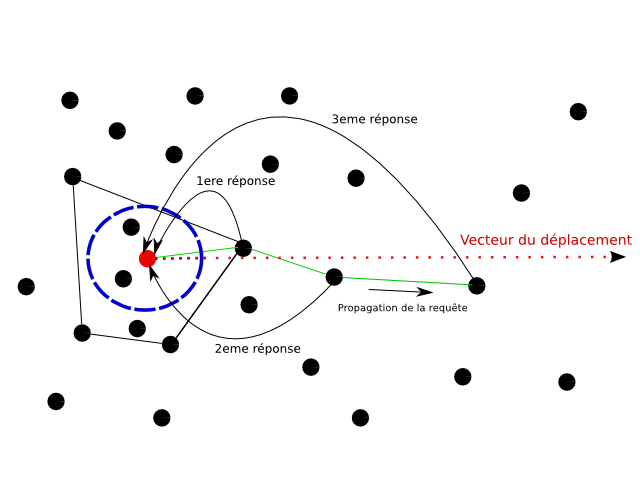
\includegraphics[scale=0.5]{../Images/propagation_algo.png}\\
        \caption{Algorithme de propagation}
        \label{Propa_Algo}
        \end{figure}
        \vspace{1cm}
\newpage
	\subsection{Expérimentations et Résultats}
		Comment ça a été testé et les résultats.
